\chapter{Diseño del Proyecto de Software}
\large{\textbf{Modelamiento Proyecto de Software (Enfoque MDA)}}
\section{CIM: Modelo Independiente de la Computaci\'on}
\subsection{Modelo de Negocio (Contexto)}
El modulo de gesti\'on de inventario a realizar constar\'a con varios componentes
entre los cuales se ver\'a el componente de acceso de usuario para el manejo del
sistema, el componente de informaci\'on de los medicamentos y el componente de
conteo de existencias, cada uno asociado al componente del gestor de la base de datos.
\newpage
\subsection{Descripción de Actores}
\begin{itemize}
\item \textbf{Gestor de informaci\'on}, ser\'a el encargado de realizar las actualizaciones de la informaci\'on de los medicamentos.
    \item \textbf{Administrador de inventario}, ser\'a el que se encargue del manejo de las cantidades de los medicamentos en la droguer\'ia.
\end{itemize}
\subsection{Diagrama de Casos de Uso}
\begin{center}
\begin{figure}[htb]
\centering
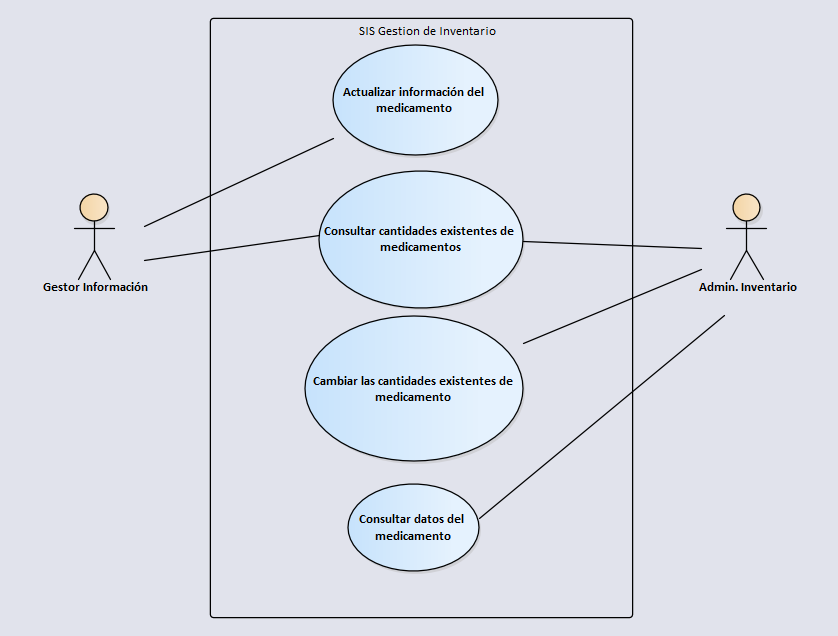
\includegraphics[width = 1.0\textwidth]{libro/capitulo5/img/CasosUso.PNG}
\caption{Diagrama de Casos de Uso - Autor\'ia propia}
\end{figure}
\end{center}
\section{PIM: Modelo Independiente de la Plataforma}
\subsection{Diagramas Estructurales}
\subsubsection{Diagrama de Clases}
123
\subsection{ Diagramas de Comportamiento}
\subsubsection{ Diagrama de Estados}

\begin{center}
    \begin{figure}[htb]
        \centering
        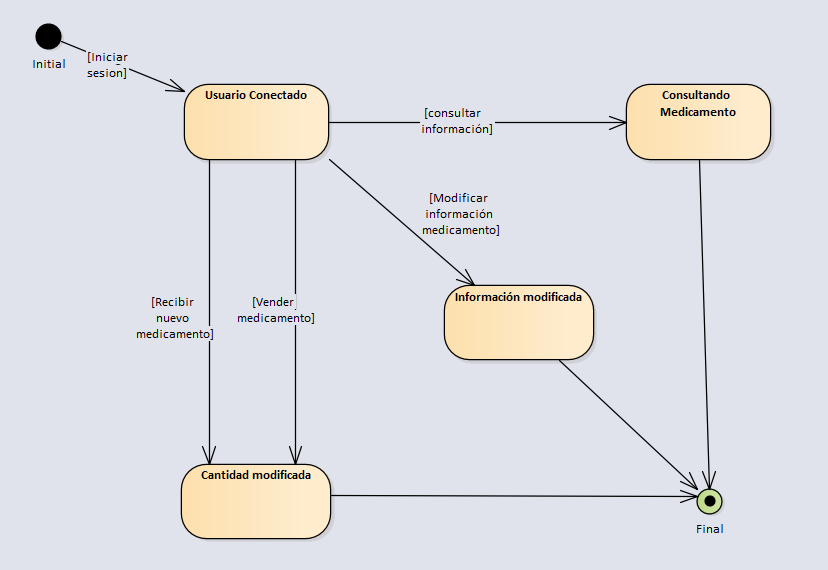
\includegraphics[width = 1.0\textwidth] {libro/capitulo5/img/Estados.PNG}
        \caption{Diagrama de Estados - Autor\'ia propia}
        \label{fig:my_label}
    \end{figure}
\end{center}
\subsubsection{ Diagrama de Actividades}
\begin{center}
    \begin{figure}[htb]
        \centering
        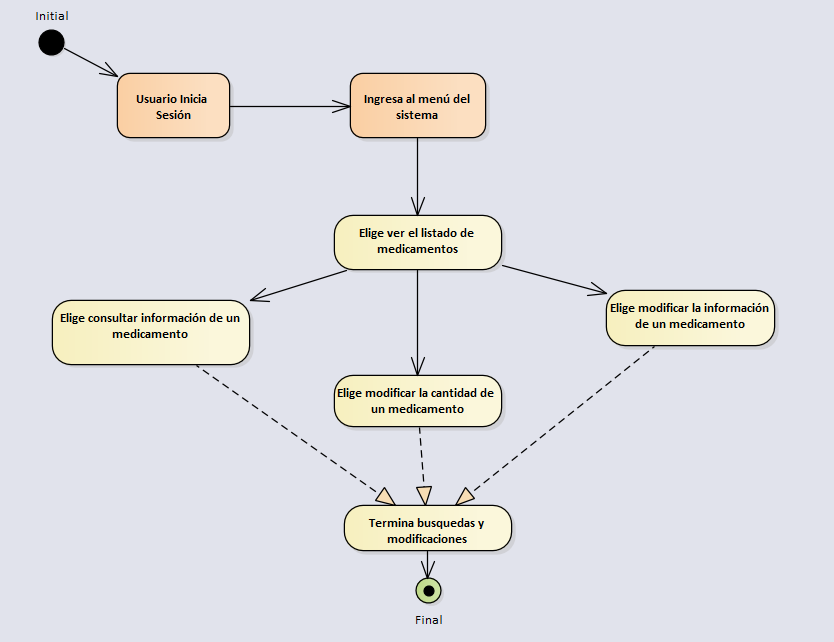
\includegraphics[width = 1.0\textwidth] {libro/capitulo5/img/Actividades.PNG}
        \caption{Diagrama de Actividades - Autor\'ia propia}
        \label{fig:my_label}
    \end{figure}
\end{center}
\subsection{ Diagramas de Interacción}
\subsubsection{ Diagrama de Secuencia}
123
\subsubsection{ Diagrama de Colaboración}
456
\subsection{ Diagramas de Implementación}
\subsubsection{ Diagrama de Componentes}
789
\subsubsection{Diagrama de Despliegue}
000
\section{PSM: Modelo Específico de Plataforma}
